Analicemos un ejemplo, moviendo 3 discos de la varilla A a la varilla C.

\begin{figure}[H]
	\centering
	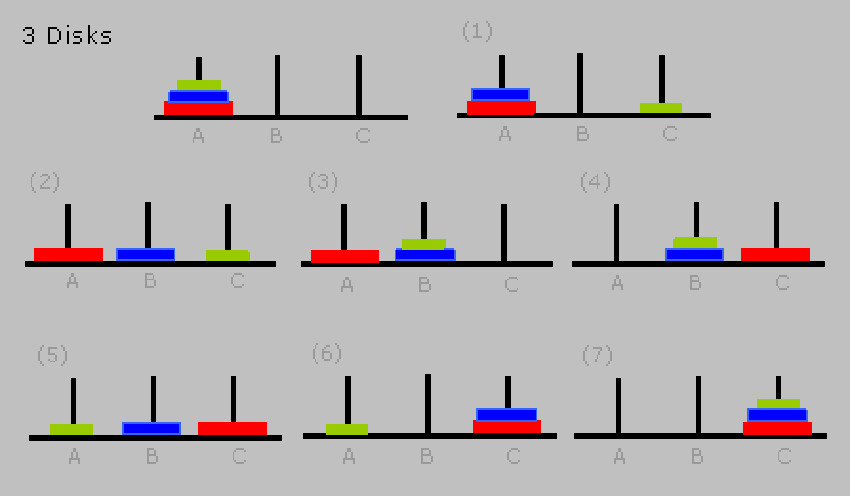
\includegraphics[width=0.9\linewidth]{cp1/hanoi3/hanoi3.jpg}
\end{figure}

Agrupemos estos pasos de manera conveniente:

\begin{figure}[H]
	\centering
	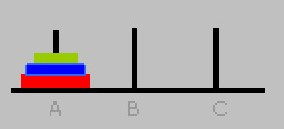
\includegraphics[width=0.45\linewidth]{cp1/hanoi3/step-0.jpg}
	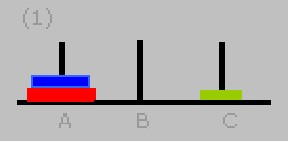
\includegraphics[width=0.41\linewidth]{cp1/hanoi3/step-1.jpg}
	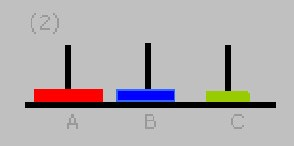
\includegraphics[width=0.45\linewidth]{cp1/hanoi3/step-2.jpg}
	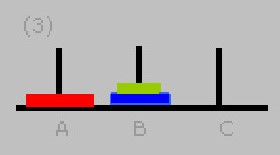
\includegraphics[width=0.41\linewidth]{cp1/hanoi3/step-3.jpg}
\end{figure}

Notemos que en este bloque de pasos (1 - 3) lo que hicimos fue mover los 2 discos más pequeños desde la varilla A hasta la varilla B usando la varilla C como auxiliar.

\begin{figure}[H]
	\centering
	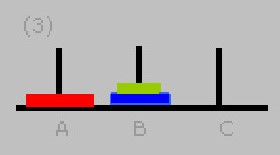
\includegraphics[width=0.42\linewidth]{cp1/hanoi3/step-3.jpg}
	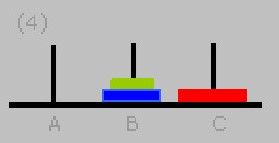
\includegraphics[width=0.45\linewidth]{cp1/hanoi3/step-4.jpg}
\end{figure}

Nos damos cuenta que en este bloque de pasos (4) lo que hicimos fue mover el disco más grande desde la varilla A hasta la varilla C.

\begin{figure}[H]
	\centering
	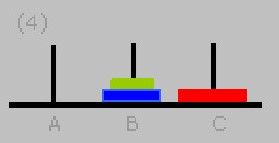
\includegraphics[width=0.45\linewidth]{cp1/hanoi3/step-4.jpg}
	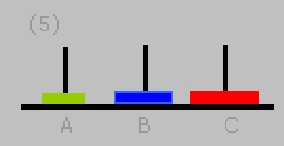
\includegraphics[width=0.45\linewidth]{cp1/hanoi3/step-5.jpg}
	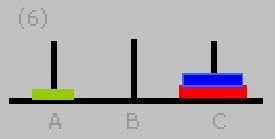
\includegraphics[width=0.45\linewidth]{cp1/hanoi3/step-6.jpg}
	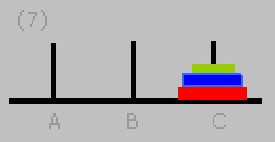
\includegraphics[width=0.44\linewidth]{cp1/hanoi3/step-7.jpg}
\end{figure}

Notemos que en este bloque de pasos (5 - 7) lo que hicimos fue mover los 2 discos más pequeños que estaban en la varilla B hasta la varilla C usando la varilla A como auxiliar.\\

\textbf{Generalizando este algoritmo, para mover $n$ discos de un poste inicial a un poste de destino, nos quedaría:}
\begin{enumerate}
    \item Mueve los $n - 1$ discos más pequeños a un poste auxiliar para liberar el disco más grande.
    \item Mueve el disco más grande al poste de destino.
    \item Mueve los $n - 1$ discos más pequeños del poste auxiliar al poste de destino, encima del disco más grande.
\end{enumerate}

Este proceso se repite para cualquier número de discos. La clave es entender que siempre estás moviendo una “torre” de discos más pequeños para liberar el disco más grande y luego reconstruir la torre en el poste de destino.\\

Llamemos $a_{n}$ al número de movimientos necesarios para mover $n$ discos de una varilla a otra, luego el procedimiento descrito nos daría la siguiente fórmula:

\[
a_{n} = a_{n - 1} + 1 + a_{n - 1}
\]

Donde:
\begin{itemize}
    \item $a_{n - 1}$ representa mover los $n - 1$ discos más pequeños al poste auxiliar.
    \item $1$ representa mover el disco más grande al poste de destino.
    \item $a_{n - 1}$ representa mover los $n - 1$ discos más pequeños del poste auxiliar al poste de destino, encima del disco más grande.
\end{itemize}

Por lo tanto, la fórmula general para el número mínimo de movimientos necesarios para resolver el problema de los $n$ discos es:

\[
a_{n } = 2 \cdot a_{n - 1} + 1
\]

Sabemos que para un disco la cantidad de movimientos necesarios es $1$, o sea $a_1 = 1$. 

Analicemos la secuencia que resulta:

\begin{itemize}
    \item Para 2 discos: $a_2 = 2 \cdot a_1 + 1 = 2 \cdot 1 + 1 = 3$
    \item Para 3 discos: $a_3 = 2 \cdot a_2 + 1 = 2 \cdot 3 + 1 = 7$
    \item Para 4 discos: $a_4 = 2 \cdot a_3 + 1 = 2 \cdot 7 + 1 = 15$
\end{itemize}

En general, para $n$ discos, el número de movimientos necesarios es:

\[
a_n = 2^n - 1
\]

Esto se puede demostrar por inducción matemática, pero lo importante ahora es entender que cada vez que agregamos un disco, duplicamos el número de movimientos necesarios y sumamos uno más.\\

Para dar respuesta a la pregunta inicial, dado que el número mínimo de movimientos necesarios para completar la tarea es:
\[
2^{64} - 1 > 18 \cdot 10^{18}
\]
Si los monjes pudieran mover un disco por segundo sin parar, les tomaría más de 584 mil millones de años completar la tarea. Así que no debemos preocuparnos más de lo que normalmente lo hacemos por este posible fin del mundo.
